\documentclass[8pt,compress]{beamer}
\usepackage{multicol}
\usepackage{graphics}
%\usepackage{cascadia-code}
\usepackage{listings}
\usepackage[default]{sourcesanspro}
\usepackage[T1]{fontenc}
\usepackage[font=tiny]{caption}
%\renewcommand*\familydefault{\ttdefault} %% Only if the base font of the document is to be typewriter style
\newcommand\LightBold[1]{\textcolor{VSBlueLight}{\textbf{#1}}}
\newcommand\DarkBold[1]{\textcolor{VSBlueDark}{\textbf{#1}}}
\newcommand\DarkBoldP[1]{\textcolor{VSPurpleDark}{\textbf{#1}}}
\usepackage[T1]{fontenc}

\usetheme{Dark}


% Title Slide
\title{Claims Investigation Committee Multi-Testing Input Device}
\subtitle{ECE-4820: Electrical and Computer Engineering Design II}
\author[Garza, Baker, Sah]{Dylan-Matthew Garza \and Daniel Baker \and Rohullah Sah \and}

\institute[VFU] % (optional)
{
      Department of Electrical and Computer Engineering\\
      Western Michigan University
      \and
      ZF Group\\
      Auburn Hills, MI
}
\date{Fall 2024}
\titlegraphic{
\includegraphics[height=2cm]{assets/WMU_Logo.png}\hspace{1cm}
\includegraphics[height=2cm]{assets/zf.png}}



\begin{document}
%==============================================================================
% Introduction slide
%==============================================================================
\begin{frame}[plain]
  \titlepage
  \small
  \begin{multicols}{2}
      Faculty Advisor:\\
      Dr. Janos Grantner\hfill\\
    \hfill{}\makebox[0pt][r]{Sponsor Manager}:\\
    \hfill Patrick McNally
  \end{multicols}
\end{frame}

\AtBeginSection[]
{
  \begin{frame}
    \frametitle{Table of Contents}
    \tableofcontents[currentsection]
  \end{frame}
}
\section{Introduction}
%==============================================================================
% INTRODUCTION SECTION
%==============================================================================
\subsection{ZF}
\begin{frame}
  \frametitle{ZF}
  \begin{minipage}{0.45\textwidth}
    \begin{block}{What is ZF?}
      \begin{itemize}
          \small {
            \item Global technology company and Tier 1 automotive supplier
            \item Provides advanced safety systems and vehicle control solutions
            \item Partners with major OEMs: Daimler, Chrysler, Tesla, Waymo(Google), etc.
            \item A leading innovator in commercial vehicle technology
          }
      \end{itemize}
    \end{block}
  \end{minipage}
  \hfill
  \begin{minipage}{0.45\textwidth}
    \begin{figure}
      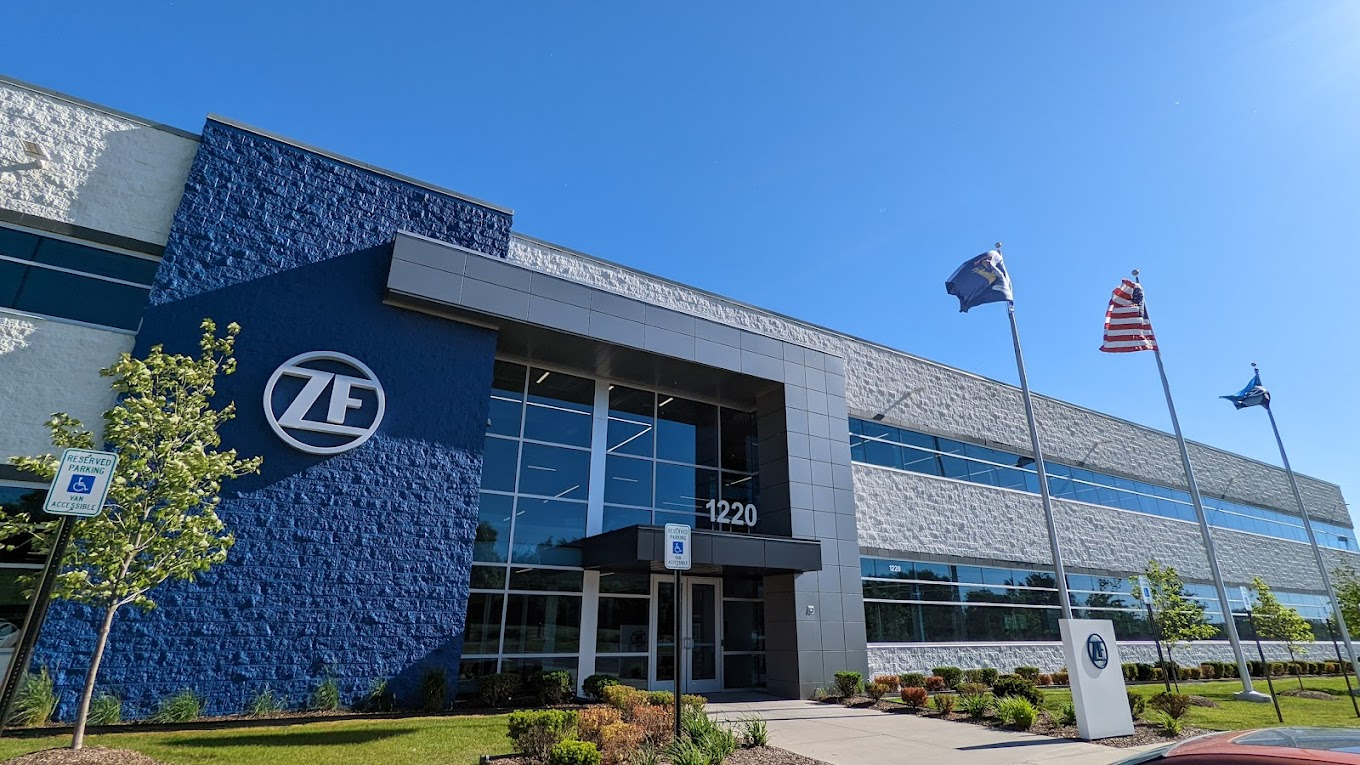
\includegraphics[width=\textwidth]{assets/misc/zf-office.jpg}
      \caption{Source: \href{google.com}{google.com}\hspace{\textwidth}
      \textit{ZF Group Office in Auburn Hills, MI}}
    \end{figure}
  \end{minipage}
  \begin{block}{Project Background}
    \begin{itemize}
        \item Claims Investigation Committee (CIC) required enhanced testing capabilities
        \item Focus on key component: Brake Signal Transmitter (BST)
        \item BST critical for highest volume commercial vehicle platform in North America (Daimler)
        \begin{itemize}
            \item Daimler Truck AG - World's largest commercial vehicle manufacturer
            \item Previous parent company of Mercedez Benz before splitting in 2021
        \end{itemize}
        \item Need for rapid, accurate analysis of field returns
    \end{itemize}
  \end{block}
\end{frame}

\subsection{Need for Multi-Testing Input Device}
\begin{frame}
    \frametitle{Need for Multi-Testing Input Device}
    \begin{block}{Project Drivers}
        \begin{itemize}
            \item BST implementation in Daimler's new platform drive urgent need
            \item Current testing methods are too time-consuming for production volumes
            \item Need for quick validation of warranty claims
            \item Opportunity to expand test capabilities to other electronic components
        \end{itemize}
    \end{block}
    %\begin{block}{Key Components Under Test}
    \begin{block}{Key Devices Under Test (DUTs)}
    \begin{enumerate}
        \item {\DarkBold{Brake Signal Transmitter (BST)}}
        \begin{itemize}
            \item Primary focus - critical new component for 2025 production
            \item Acts as the brain that reads how hard a driver presses the brake.
        \end{itemize}
        \item {\DarkBold{Continuous Wear Sensor (CWS)}}
        \begin{itemize}
            \item Works like a monitor for your brake pads and discs
            \item Warns when brakes are wearing down using voltage
        \end{itemize}
        \item {\DarkBold{Pressure Sensor}}
        \begin{itemize}
            \item Continuously measures relative pressure in vehicle control systems
        \end{itemize}
        \item {\DarkBold{Electronic Stability Control Module (ESCM)}}
            \begin{itemize}
                \item Acts as a safety system that helps prevent skidding and rollovers
                \item Monitors the vehicle's movement and intervenes to keep it stable
            \end{itemize}
    \end{enumerate}
  \end{block}
\end{frame}

%==============================================================================
% DESIGN AND IMPLEMENTATION SECTION: Project Specifications and Overview
%==============================================================================

\section{Design and Implementation}
\subsection{Project Specifications and Overview}

\begin{frame}
  \frametitle{Project Specifications}
  \large
  \begin{block}{What this project aims to accomplish:}
    \begin{enumerate}
      \item {\DarkBold{Device Interfacing}}
        \begin{enumerate}
          \large
          \item Properly read Device Signals using the ARM Cortex-M4 on the onboard microcontroller on the 
            \LightBold{STM32MP157F-DK2}:
            \begin{itemize}
              \large
              \item PWM Duty Cycle
              \item Frequency
              \item Voltages through an analog-to-digital converter (ADC)
              \item CAN frames
            \end{itemize}
        \end{enumerate}
    \end{enumerate}
  \end{block}
\end{frame}

\begin{frame}
  \frametitle{Project Specifications (cont.)}
  \large
  \begin{block}{Project Specifications}
    \large
    \begin{enumerate}
        \setcounter{enumi}{1}
      \item \DarkBold{Physical Components and Hardware}
        \begin{enumerate}
          \large
          \item Printed Circuit Board (PCB) for interfacing with DUT
          \item PCB for scaling and managing power for the DUT and to the microcontroller
          \item Enclosure for PCBs and \LightBold{STM32MP157F-DK2} board
        \end{enumerate}
    \end{enumerate}
  \end{block}
\end{frame}

\begin{frame}
  \frametitle{Project Specifications (cont.)}
  \begin{block}{What this project aims to accomplish:}
    \begin{enumerate}
        \setcounter{enumi}{2}
        \large
      \item \DarkBold{Software}
        \begin{enumerate}
            \large
          \item Custom embedded \textbf{Linux} distribution that will run on the onboard ARM Cortex-A7
            microprocessor on the \LightBold{STM32MP157F-DK2}
          \item Simple user interface web-based application
          \item Custom Webserver to process information from web application to microcontroller
          \item Communicate collected information from ARM Cortex-M4 to ARM Cortex-A7
          \item Ability to download measured data, formatted as a CSV, through the web application 
        \end{enumerate}
    \end{enumerate}
  \end{block}
\end{frame}

%==============================================================================
% DESIGN AND IMPLEMENTATION SECTION: Gantt Chart
%==============================================================================
\begin{frame}
  \frametitle{Gantt Chart}
  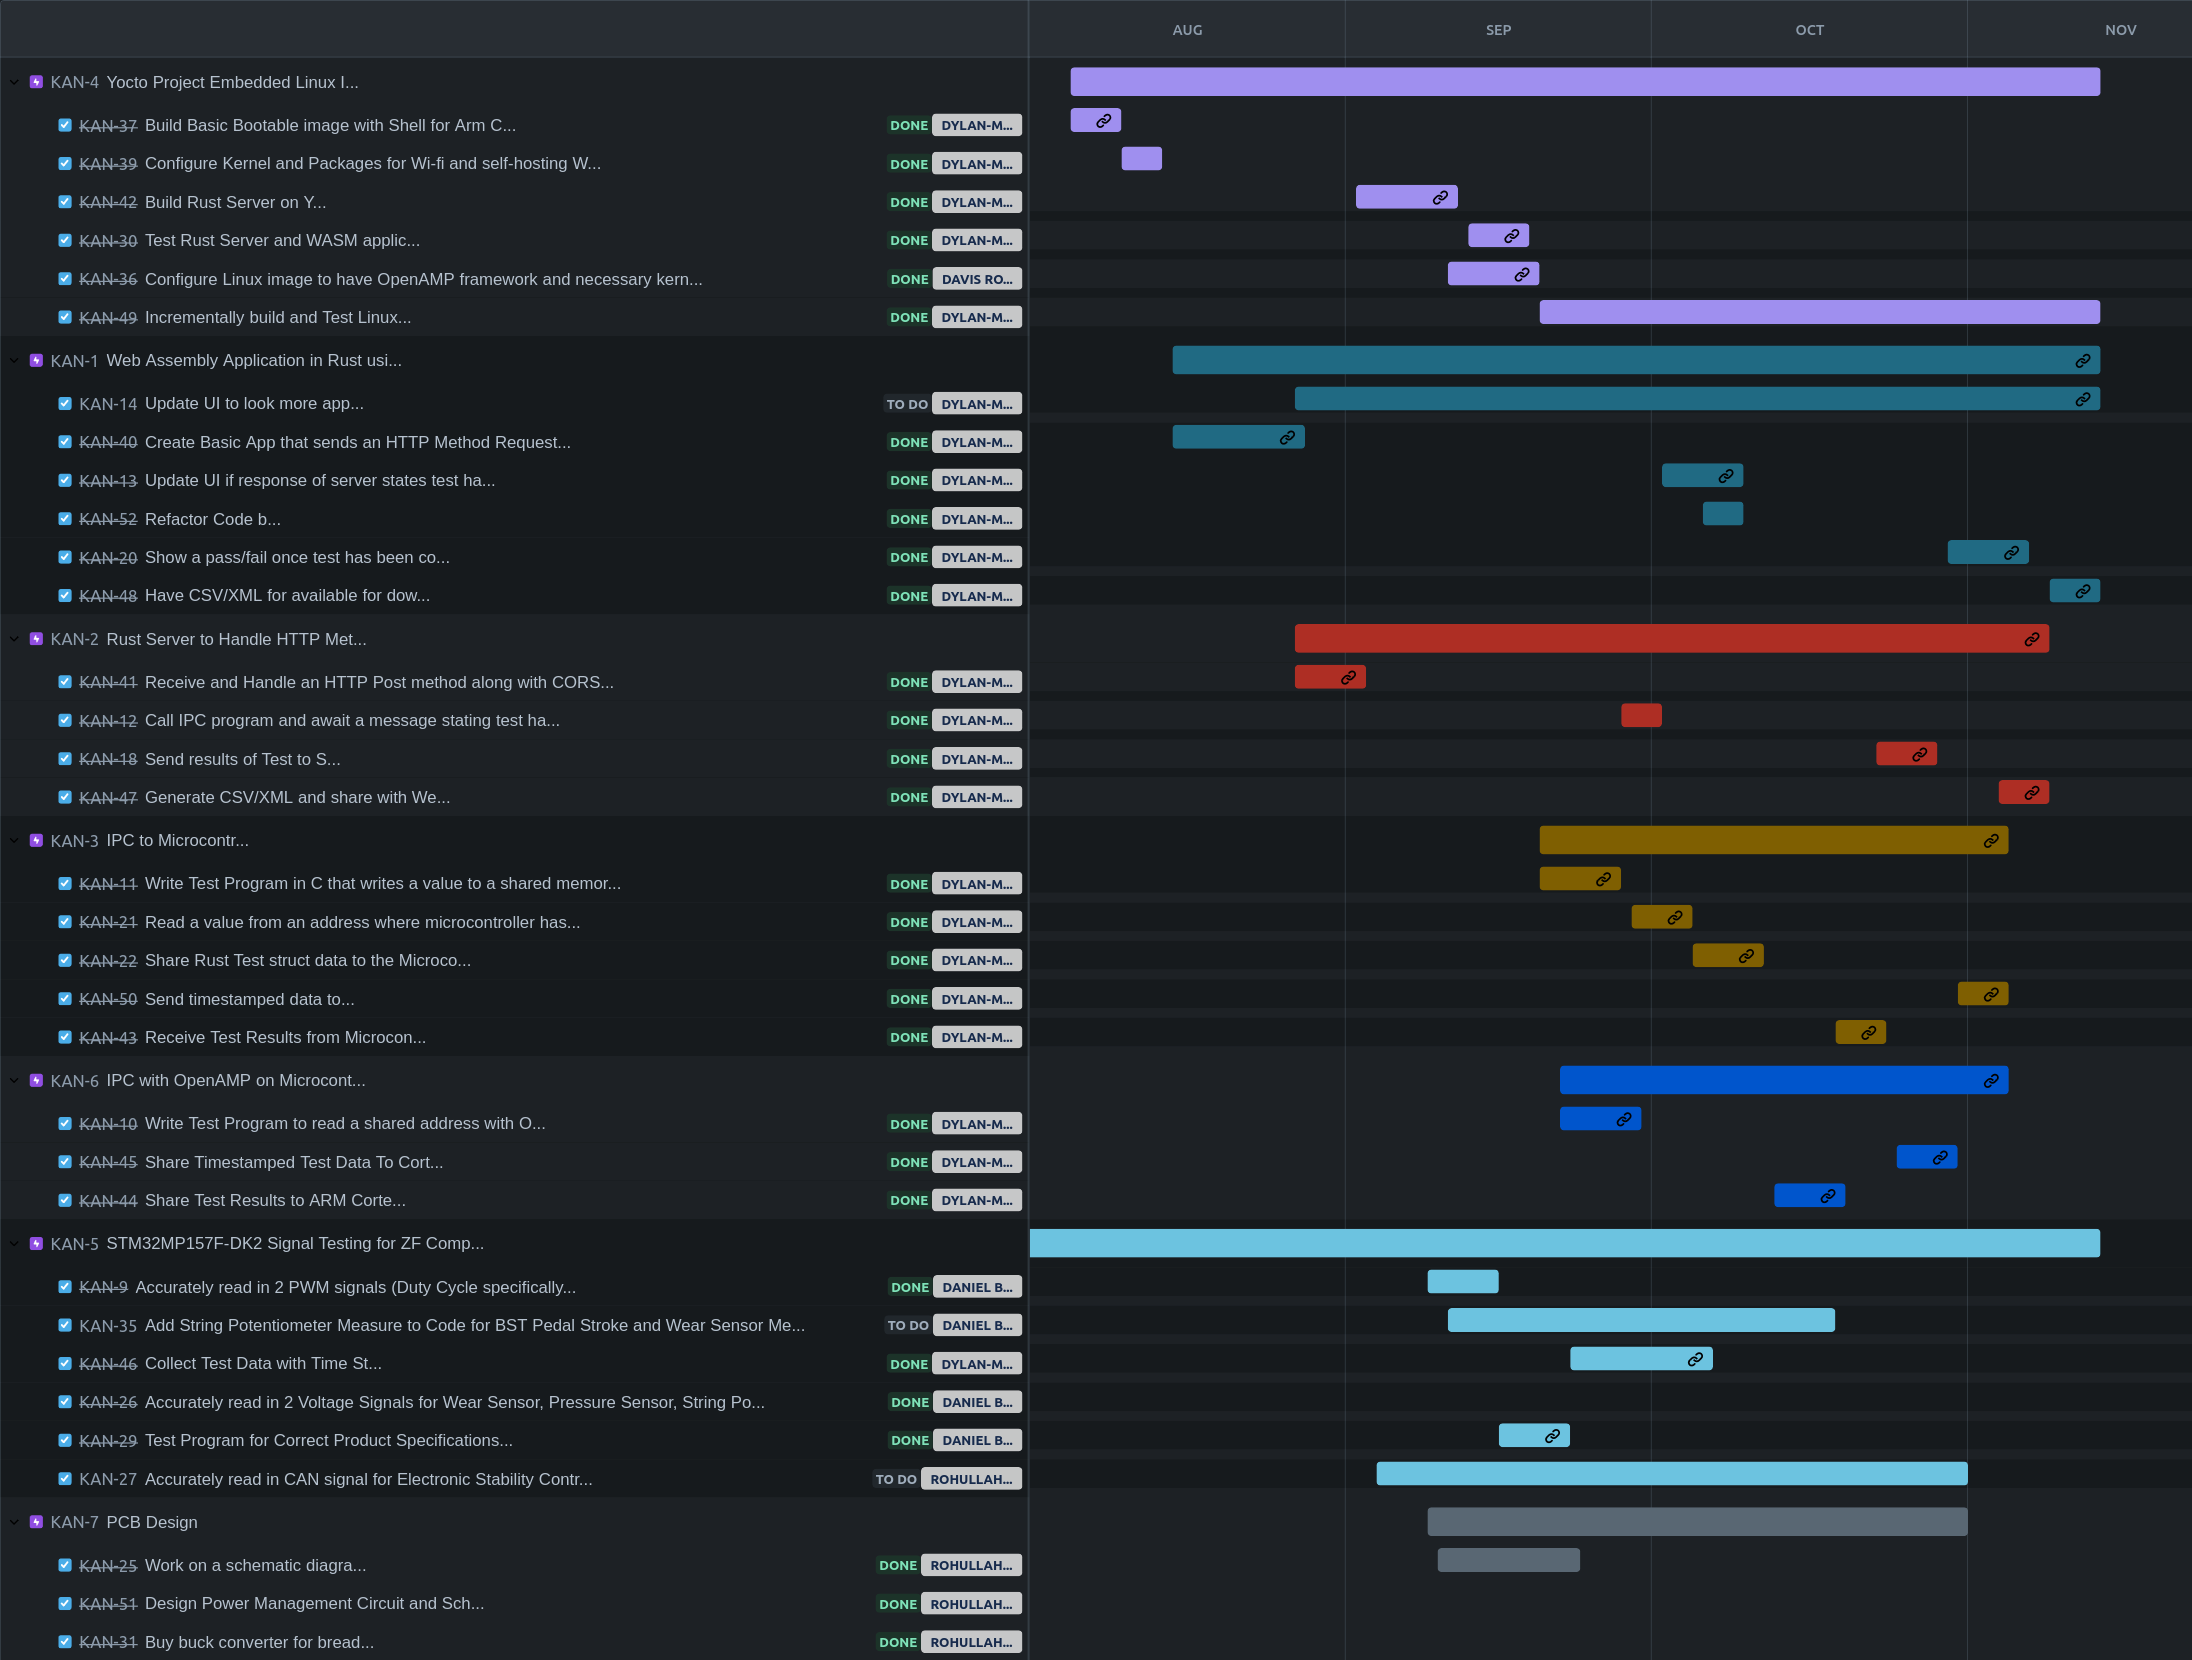
\includegraphics[width=0.875\textwidth]{assets/diagrams/gantt.png}
\end{frame}
%==============================================================================
% DESIGN AND IMPLEMENTATION SECTION: Budget Projection
%==============================================================================
\begin{frame}
  \frametitle{Budget Projection}
  \vspace{-.2025cm}
  %\includegraphics[height=\dimexpr\paperheight-1.825cm\relax]{assets/diagrams/}
\end{frame}

%==============================================================================
% DESIGN AND IMPLEMENTATION SECTION: Hardware Design
%==============================================================================
% Talk about the need and design of custom hardware (eg. simplify wiring, scale voltages for microcontroller
%   simplify connectivity, pull-up resistor network for BST)
\AtBeginSubsection[]
{
  \begin{frame}
    \frametitle{Table of Contents}
    \tableofcontents[currentsubsection]
  \end{frame}
}


\subsection{Hardware Design}
\begin{frame}
  \centering
  \frametitle{Custom Hardware Design}
\end{frame}

%==============================================================================
% DESIGN AND IMPLEMENTATION SECTION: Cortex-M4 Firmware
%==============================================================================
\subsection{Cortex-M4 Firmware to Test Devices}
\begin{frame}
  \frametitle{Firmware to Test Brake Signal Transmitter (BST)}
  \begin{block}{Purpose}
    \small{
      \begin{itemize}
        \item Developed firmware on the onboard Cortex-M4 microcontroller to validate BST
        \item Ensures accurate detection of how hard a driver presses the brake pedal
       %\item Ensures brake actuation is accurate to distance moved by brake pedal
       % ^suggested change
      \end{itemize}
    }
  \end{block}
  \hspace{-0.5cm}
  \begin{minipage}{0.485\textwidth}
    \begin{block}{Method}
      \small{
        \begin{itemize}
          \item \LightBold{Input Capture:} Timers captures read two PWM signals from the BST
          \item \LightBold{ADC Reading:}Optional string potentiometer for direct analog voltage measurements via ADC 
            %^ADC already defined in project specification, "converter" after ADC is redundant
          \item \LightBold{Processing:} Calculates duty cycles, frequencies, and estimated stroke via timer interrupts
            %^changed "readings" to "interrupts"
          \item \LightBold{Validation:} Compare measurements against expected values according to product specifications to verify BST accuracy
          \item \LightBold{Results:} Sends test results to the main processor for logging and user display
        \end{itemize}
      }
    \end{block}
  \end{minipage}
  \hfill
  \begin{minipage}{0.50\textwidth}
    \begin{figure}
      \centering
      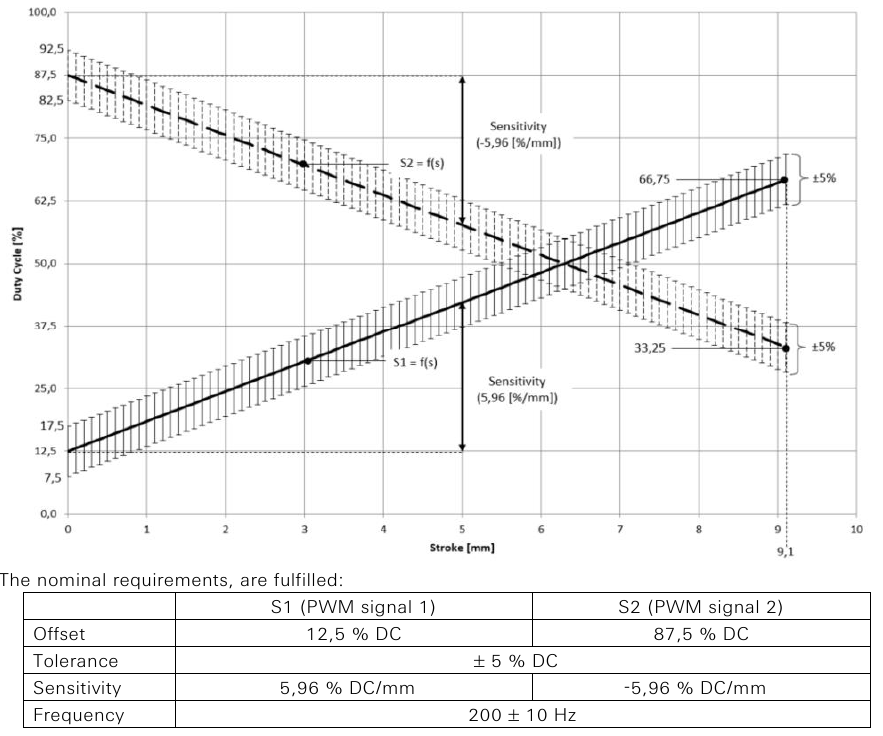
\includegraphics[width=\textwidth]{assets/specs/bst_product_specs.png}
      \caption{\it Product Specifications for BST}
    \end{figure}
  \end{minipage}
\end{frame}
% CWS Test implementation
\begin{frame}
  \frametitle{Firmware to Test Continuous Wear Sensor (CWS)}
\end{frame}

% Pressure Sensor Test Implementation
\begin{frame}
  \frametitle{Firmware to Test Pressure Sensor}
\end{frame}

%==============================================================================
% DESIGN AND IMPLEMENTATION SECTION: Embedded Linux
%==============================================================================
\subsection{Embedded Linux With Yocto Project}
\begin{frame}
  \frametitle{Embedded Linux}
  \begin{figure}
    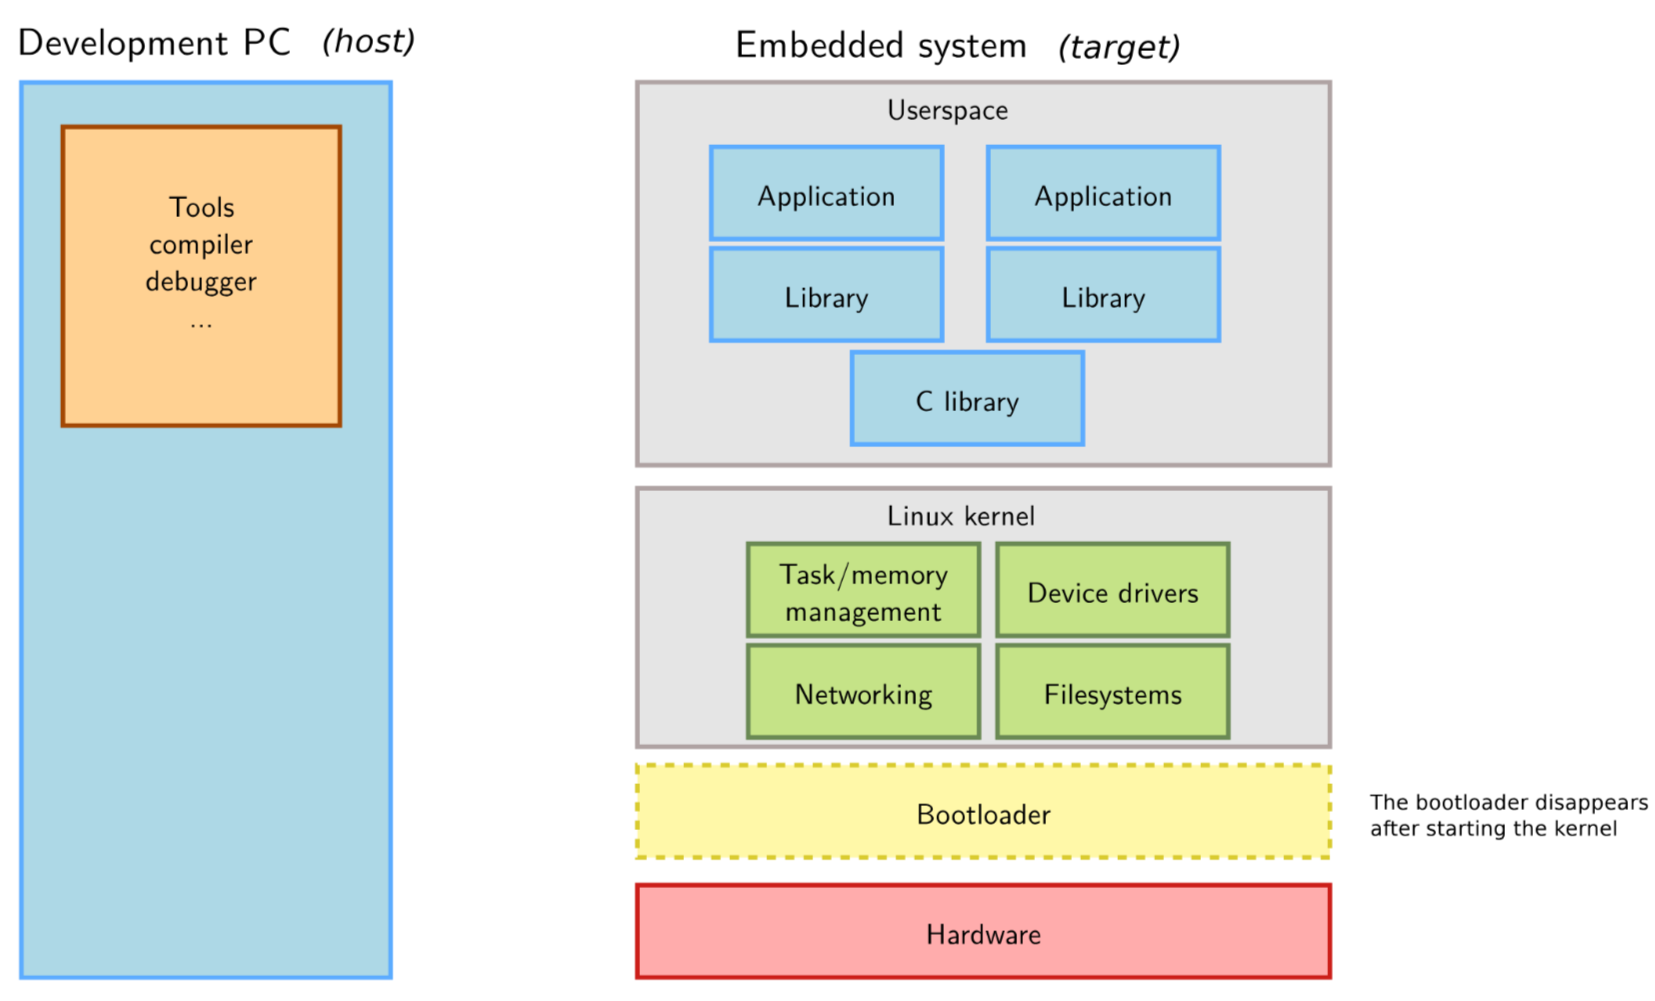
\includegraphics[width=175px]{assets/diagrams/embedded_linux.png}
    \centering
    \caption{\tiny Source:\underline{\href{https://bootlin.com/}{https://bootlin.com/}}\hspace{\textwidth}
    \textit{Embedded Linux system architecture}}
  \end{figure}
  \vspace{-16px}
  \begin{block}{Why use embedded Linux?}
    \small{
      \begin{itemize}
        \item Industry standard for any embedded operating system
        \item Access to open-source software (OSS) and tools
        \item Networking and connectivity made easy 
        \item Easily save/access data with filesystem
      \end{itemize}
    }
  \end{block}
\end{frame}

\begin{frame}
  \frametitle{Using The Yocto Project to Build a Custom Distribution}
    \begin{block}{What is the Yocto Project and why?}
      {
        \begin{itemize}
          \item Most popular set of tools for embedded Linux Development
          \item Collection of OSS tools to make a custom Linux distribution
          \item Independent of target architecture
          \item \DarkBoldP{bitbake} build tool handles \LightBold{metadata}
          \item \LightBold{MetaData} can be in the form of 
            \begin{itemize}
              \item software build/patch instructions
              \item configuration files for software
            \end{itemize}
          \item \LightBold{MetaData} organized in its \LightBold{Layer Model}
        \end{itemize}
      }
    \end{block}
  \hfill
    \vspace{-12px}
    \center
    \begin{figure}
      \center
      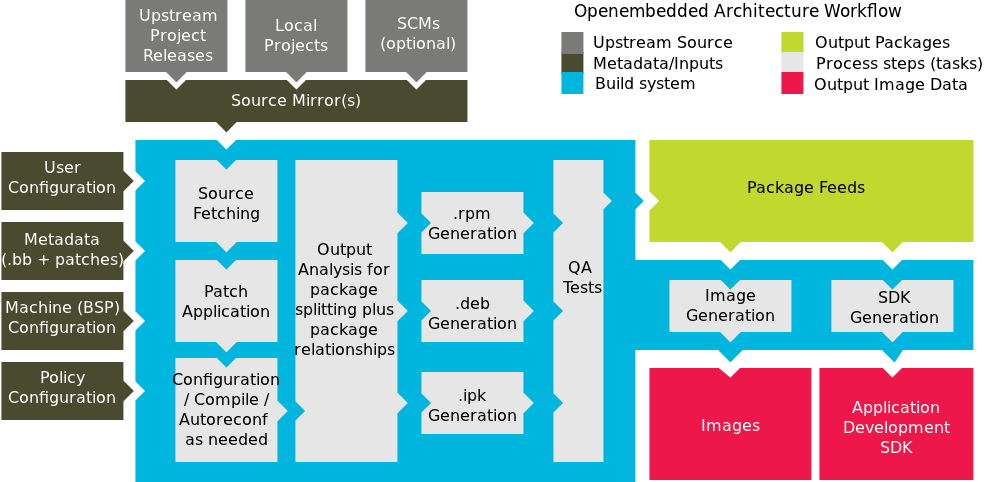
\includegraphics[width=180px]{assets/diagrams/yocto-environment.png}
      \caption{Source: \href{https://docs.yoctoproject.org}{https://docs.yoctoproject.org}\hspace{\textwidth}
      \it High-level diagram representing how builds work using The Yocto Project}
    \end{figure}
\end{frame}

\begin{frame}
  \frametitle{Custom Linux Image for the STM32MP1-DK2}
  \begin{minipage}{0.475\textwidth}
    \begin{block}{What is used in the deployed image?}
      \begin{itemize}
        \item ST's BSP (board support package) layer provides metadata 
          \begin{itemize}
            \small
            \item Hardware drivers
            \item Kernel Configurations
            \item Devicetree
          \end{itemize}
        \item Custom layer \DarkBoldP{meta-zf-project}
          \begin{itemize}
            \small
            \item \DarkBold{nginx} (webserver), \DarkBold{wpa\_supplicant} (Wi-Fi access client/
              IEEE 802.1X supplicant)
            \item recipes for custom applications (Web application, Server, Cortex-M4 Firmware)
            \item Kernel configurations and custom Devicetree
          \end{itemize}
      \end{itemize}
    \end{block}
  \end{minipage}
  \hfill
  \begin{minipage}{0.5\textwidth}
    \begin{figure}
      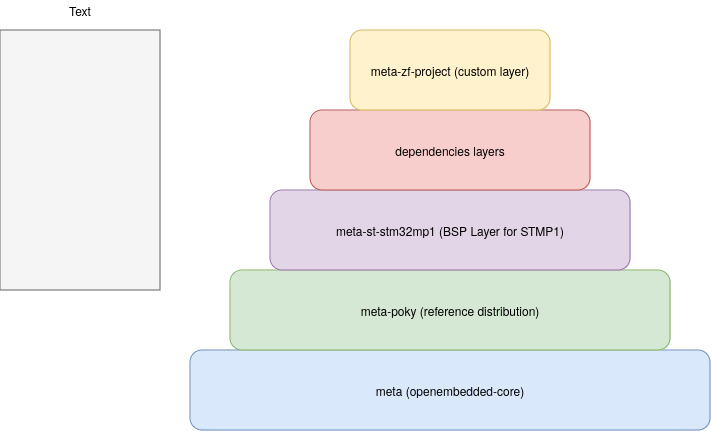
\includegraphics[width=1.125\textwidth]{assets/diagrams/layers.png}
      \caption{\it Layer Model representation of this project for deploying onto a 
      STM32MP1-DK2}
    \end{figure}
  \end{minipage}
\end{frame}

%==============================================================================
% DESIGN AND IMPLEMENTATION SECTION: IPC with OpenAMP
%==============================================================================
\subsection{Inter-Processor Communication}
\begin{frame}
  \frametitle{Inter-Process Communication on a Heterogenous Architecture}
  With a heterogenous architecture (ARM Cortex-A7 and ARM Cortex-M4) how can information be shared?\\
  {\em \scriptsize Hetergenous multiprocessor SoCs cannot directly communicate }
  \break
  \begin{minipage}{0.465\textwidth}
    \begin{block}{OpenAMP (Asymmetric Multi-Processing) Project}
      \footnotesize
      \begin{itemize}
        \item Software framework that places standard protocol for shared memory
        \item Implemented on top of \DarkBoldP{virtio} framework
        \item STM provides \DarkBoldP{virt\_uart} driver for recieving/transmitting messages
          over \DarkBoldP{RPMsg protocol}
        \item STMP1 layer automatically enables the \DarkBoldP{RPMSG tty driver} kernel module
          \begin{itemize}
              \tiny
            \item creates file in Linux filesystem: \DarkBoldP{/dev/ttyRPMSG<X>}
            \item can read and write to like a normal file
          \end{itemize}
        \item \DarkBoldP{remoteproc} framework allows dynamic and remote loading of Cortex-M4 firmware
        \item \LightBold{Resource Table} defined in firmware opens a trace in\\
          {\scriptsize\DarkBoldP{/sys/kernel/debug/remoteproc/remoteproc0/trace0}}
          \begin{itemize}
              \tiny
            \item Used for logging measured data in CSV format
          \end{itemize}
      \end{itemize}
    \end{block}
  \end{minipage}
  \hfill
  \begin{minipage}{0.465\textwidth}
    \begin{figure}
      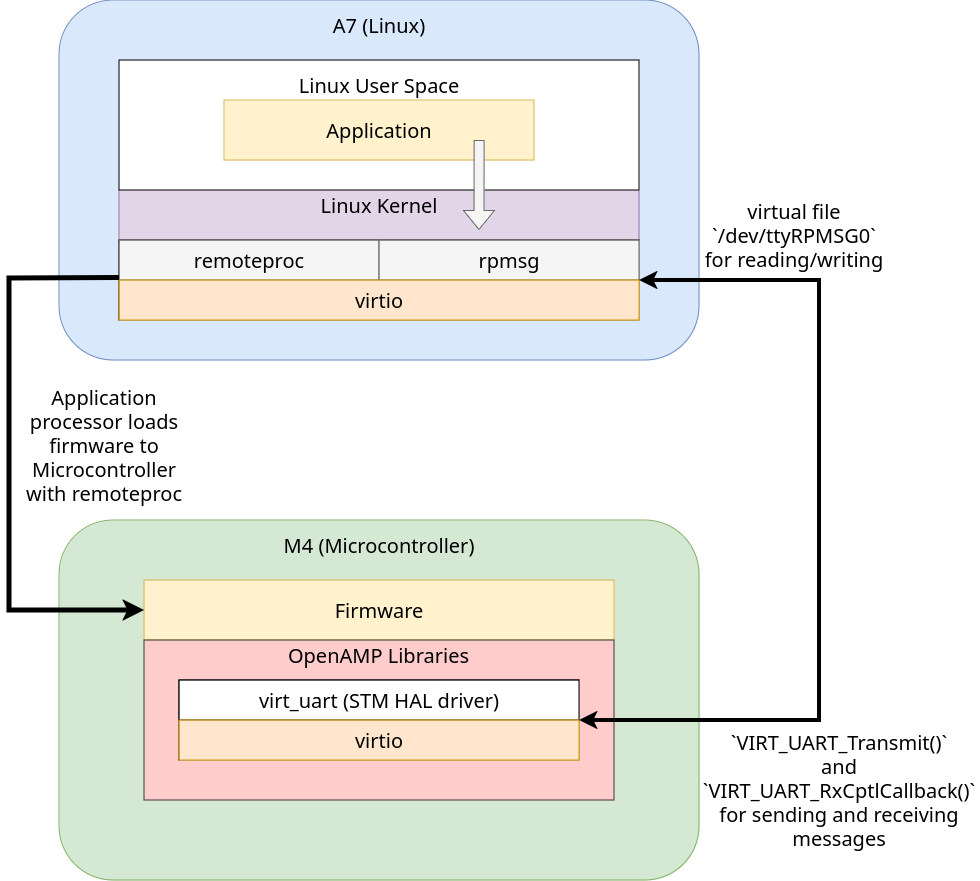
\includegraphics[width=\textwidth]{assets/diagrams/ipc.drawio.png}
      \caption{IPC between Linux (A7) and Microcontroller (M4)}
    \end{figure}
  \end{minipage}
\end{frame}



\end{document}
